\chapter{Proposed Methodology}
\label{chap:methodology}
This chapter describes the proposed meta-heuristic to solve the MSSC problem. The designed method is based on a genetic algorithm (GA) with local improvements combined with mechanisms that allow the diversification of the population (local minima escape) and the propagation of good solutions. In this method, the local improvement procedure is performed via the running of the K-means algorithm, which takes one candidate solution in the GA population as a starting point. In other words, the method may be defined as a multi-start K-means inside a GA framework, which in turn is guided by the MSSC objective. 

\section{General structure}
\label{sec:general-structure}
The GA here proposed works through the following simple cycle of stages:

\begin{enumerate}
	\item Creation of an initial population of individuals (candidate solutions);

	\item Selection of parents;

	\item Genetic manipulation to create new individuals (crossover and mutation);
	
	\item Enhancement of the produced individual (local improvement);
	
	\item Selection of survivors individuals for propagation.
	
\end{enumerate}

This general scheme of the meta-heuristic is described in more details by Algorithm \ref{genetic-algo}. Initially, the method generates a random population of individuals (see \ref{sec:initial-population}). A population is a set of solutions, where each individual represents a point in a search space of the optimization problem. Then, it applies successively a number of operators to evolve this population. Firstly, it selects two parent individuals (see \ref{subsec:selection}) from the population and combines them by a crossover procedure (see \ref{subsec:crossover}), yielding to a new individual (offspring) that is added to the population. Secondly, the offspring is mutated (see \ref{subsec:mutation}) and enhanced by a local improvement (see \ref{subsec:local-improvement}), generating a new individual solution that is also added to the population. These two steps -- crossover and mutation with enhancement -- are performed many times until a termination criteria is reached.

In addition to the genetic operators mentioned above, a mechanism to select the survivor individuals is applied when a pre-defined criteria is reached (see \ref{sec:population-management}). This mechanism allows the method to propagate the best individuals and keep the diversity of the population. The following sub-sections describes how these operators and mechanisms to evolve and manage the population of solutions work.

\begin{algorithm}[!h]
\caption{Genetic algorithm framework}
\label{genetic-algo}
\begin{algorithmic}[1]
\STATE Initialize population
\WHILE{number of iterations without improvement $< I_{S}$ and $I_{max}$ not reached}
\STATE Select parents $p_1$ and $p_2$
\STATE Generate an offspring $\theta$ from $p_1$ and $p_2$ (crossover)
\STATE Generate an individual $\theta'$ by mutating $\theta$ (mutation)
\STATE Apply local improvement on $\theta'$
\STATE Add $\theta$ and $\theta'$ to the population
\IF{population size is equal to the maximum size $\Pi$ of population}
\STATE Select survivors
%\IF{best solution not improved for $I_D$ iterations}
%\STATE Diversify population
%\ENDIF
\ENDIF
\ENDWHILE
\STATE Return best solution
\end{algorithmic}
\end{algorithm}

\section{Solution representation}
\label{sec:solution-representation}
A solution (clustering partition) is represented by two direct encodings: (i) the point-cluster assignment and (ii) the centroids description. The idea of the point-cluster assignment is to use a genetic encoding that allocates directly $n$ data points to $m$ clusters, such that each candidate solution consists of a $n$-vector ($n$ genes) with integer values in the interval [1, $m$]. Thus, for $n$ = 4 and $m$ = 3, the encoding (1,1,3,2) allocates the first and the second data points to cluster 1; the third data point to cluster 3 and the fourth data point to cluster 2, generating the partition (\{1,2\}, \{4\}, \{3\}).

\begin{figure}[h]
  \begin{center}
    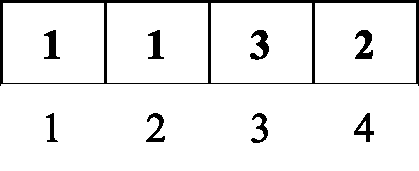
\includegraphics[width=0.3\textwidth]{img/assignment-encoding}
    \caption{Assignment encoding for $n$ = 4 and $m$ = 3}\label{fig:assignment-encoding}
  \end{center}
\end{figure}

The encoding based on the centroids description defines a solution through the feature vectors existing in each centroid. A solution is represented by a matrix $C$ of size $m \times d$, where $m$ is the number of centroids (clusters), $d$ is the number of features and an entry $c_{ij}$ of $C$ is the value of the $j$-th feature of the $i$-th centroid ($i$ = 1 ... $m$; $j$ = 1 ... $d$) (see Figure \ref{fig:centroids-encoding}).

\begin{figure}[h]
  \begin{center}
    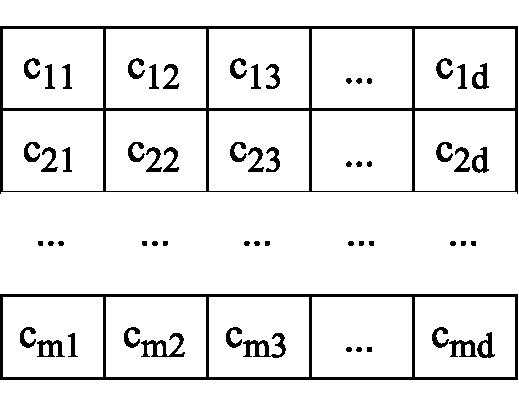
\includegraphics[width=0.4\textwidth]{img/centroids-encoding}
    \caption{Encoding based on centroids features}\label{fig:centroids-encoding}
  \end{center}
\end{figure}

\section{Initial population}
\label{sec:initial-population}
The first step in a GA is the generation of an initial population. It has been recognized that if the initial population of the GA is good, then the algorithm has a greater possibility of finding a good solution \cite{Burke2004, Zitzler2000}. In this work, the initial population is randomly generated, by assigning each data point to a cluster according to a discrete uniform distribution, i.e., where each outcome is equally likely to happen. To compose the initial population, 100 individuals are created. Then, each initial individual is submitted to the local improvement. Some factors can influence the initial population or should be taken into account when an initial population is generated randomly: the search space, the fitness function, the diversity, and the number of individuals \cite{DiazGomez2007}.

\section{Individuals management}
\label{individuals-management}
In order to increase the population and propagate good solutions, the algorithm needs to keep introducing new individuals. The generation of a new individual (offspring) begins with the random selection of two parents, $p_1$ and $p_2$, which are submitted to a crossover procedure that generates a child individual $\theta$. Then, $\theta$ is added to the population. As highly fit solutions have more chances to be selected for reproduction, the offspring -- which combines characteristics from each parent -- is likely to have a good fitness. Thus, we also consider the mutation operator, which generates a new individual $\theta'$ that is similar to $\theta$ and tends to be good regarding the fitness.

\subsection{Selection}
\label{subsec:selection}
The selection is the stage where individuals from the population are chosen to mate and generate a new individual. Due to the evolutionary behaviour of GA, the most likely individuals to be chosen for selection are the ones with good fitness. That way, good fragments of solutions can be propagated to generate good children solutions. In the proposed method, the parent selection is done through a \textit{w}-tournament, which randomly selects $w$ individuals (in a discrete uniform distribution) from the population and keeps the one with the best fitness among the $w$ individuals to set the first parent. The fitness here considered is the value of the objective function (cost) of a solution. Then, the same selection scheme is performed for the second parent. The value of $w$ was chosen according to a calibration process described in Section \ref{sec:calibration}.

\subsection{Crossover}
\label{subsec:crossover}
Once parent solutions $p_1$ and $p_2$ were selected, they are submitted to a crossover procedure in order to produce a offspring (child) solution. The crossover operator works as follows:

\begin{enumerate}
	%\item Firstly, the minimum bipartite matching between centroids of $p_1$ and $p_2$ is found. Given a graph $G = (V_1, V_2, E)$, where $V_1$ is the set of centroids (nodes) of parent $p_1$, $V_2$ is the set of centroids of parent $p_2$, and $c_{ij} \in E$ is the euclidean distance for every $i \in V_1$ and $j \in V_2$; the goal is to find a one-to-one matching $M$ such that the sum of the values of the edges in $M$ is minimum. In other words, the goal is to produce the one-to-one assignment of centroids from different sets (parents), in such a way that the sum of all distances considered in the assignment is minimized. This matching problem is solved by the Hungarian method \cite{Kuhn1955} and leads to $m$ pairs of centroids, where $m$ is the number of clusters (centroids).

	\item Firstly, a solution for the minimum weighted bipartite matching between centroids of $p_1$ and $p_2$ is found (Figure \ref{fig:crossover} (b)). Finding such a matching is known as the assignment problem. Let $G = (V, E)$ be a complete bipartite graph whose node set can be partitioned as $V = X \cup Y$, with the property that every edge $e \in E$ has one end in $X$ and the other in $Y$, and every node of $X$ is connected to every node of $Y$. Consider also that $|X| = |Y| = m$. An assignment $M$ in $G$ is the subset of edges $M \subseteq E$ of minimum cost, such that each node appears in exactly one edge in $M$ \cite{tardos}. In our case, the nodes in $X$ and $Y$ correspond to the centroids of $p_1$ and $p_2$, respectively. The cost of an edge $e \in E$ is the Euclidean distance between two centroids $c' \in X$ and $c'' \in Y$. Thus, the objective is to produce the one-to-one assignment of centroids from different sets (parents), in such a way that the sum of all distances considered in the assignment is minimized. In other words, we aim to join the similar centroids of different individuals. We solve this matching problem with the Hungarian algorithm \cite{Kuhn1955}, using the specific implementation of \textit{dlib} C++ library (King, 2011), which works with a complexity of $O(m^3)$ and leads to $m$ pairs of centroids, where $m$ is the number of clusters (centroids).

%One set of nodes in the matching problem is composed by the centroids of $p_1$ and the other set is composed by the centroids of $p_2$. The goal is to produce the one-to-one assignment of centroids from different sets, in such a way that the overall edges weight (distances) is minimized.

	\item For each pair of centroids resulted from the assignment solution, one of them is randomly selected (Figure \ref{fig:crossover} (c)) and set as a centroid of the offspring, resulting in a solution with $m$ centroids, each coming from $p_1$ or $p_2$ (Figure \ref{fig:crossover} (d)).

	\item Finally, data points are assigned to the closest offspring centroid.
\end{enumerate}

%\begin{figure}[H]
%  \begin{center}
%    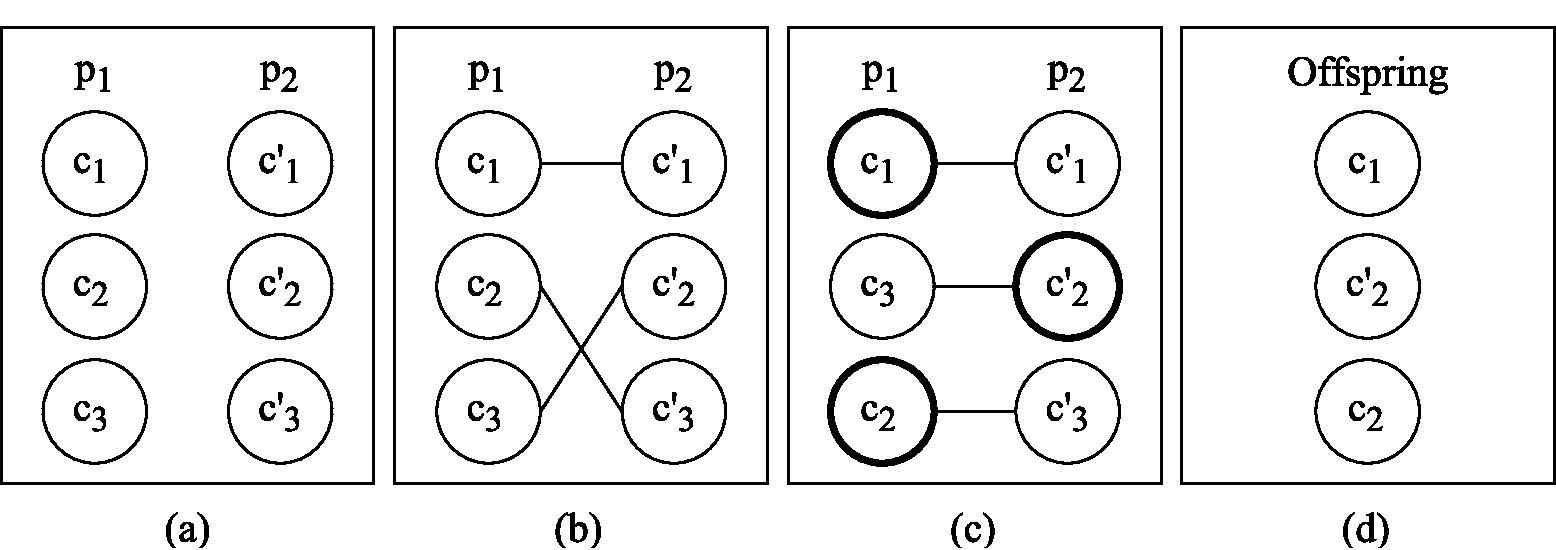
\includegraphics[width=1.0\textwidth]{img/crossover}
%    \caption{Crossover based on centroids matching: (a) two parent solutions; (b) the assignment between centroids of $p_1$ and $p_2$; (c) random selection of matched centroids and (d) the produced offspring.}\label{fig:crossover}
%  \end{center}
%\end{figure}

\begin{figure}[H]
\centering
\subfigure[Parents $p_1$ and $p_2$]{\label{fig:crossoverA}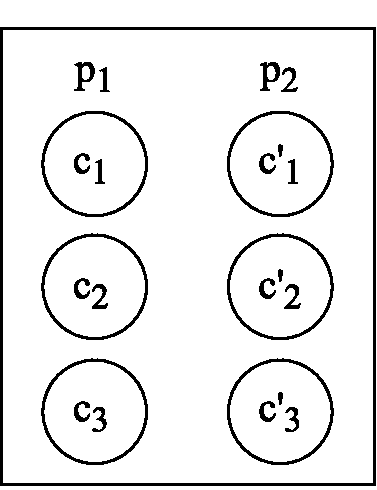
\includegraphics[width=0.24\textwidth]{img/crossoverA}}
\subfigure[Assignment]{\label{fig:crossoverB}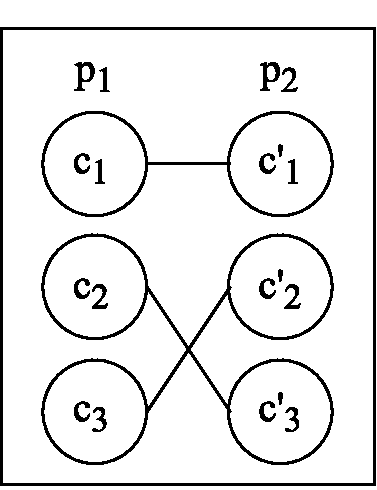
\includegraphics[width=0.24\textwidth]{img/crossoverB}}
\subfigure[Random selection]{\label{fig:crossoverC}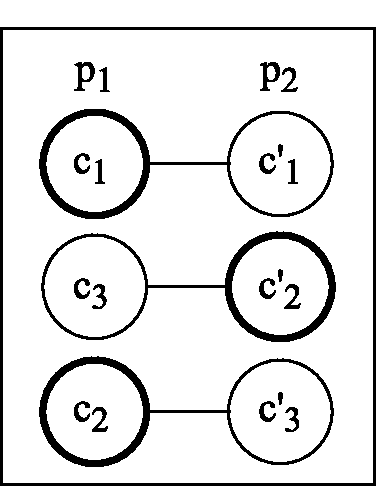
\includegraphics[width=0.24\textwidth]{img/crossoverC}}
\subfigure[New solution]{\label{fig:crossoverD}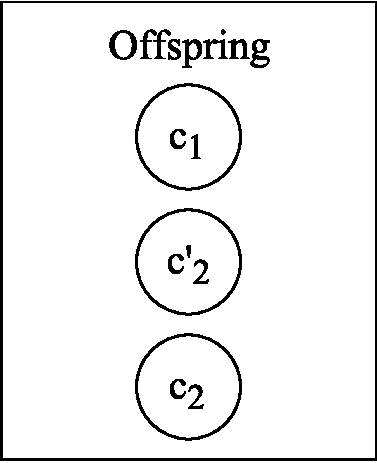
\includegraphics[width=0.24\textwidth]{img/crossoverD}}
\caption{Crossover based on centroids matching: (a) two parent solutions; (b) the assignment between centroids of $p_1$ and $p_2$; (c) random selection of matched centroids and (d) the produced offspring}
\label{fig:crossover}
\end{figure}

%Given a graph $G = (V_1 \union V_2, E)$, where $V_1$ is the set of centroids (nodes) of parent $p_1$, $V_2$ is the set of centroids of parent $p_2$, and an edge $e_{ij} \in E$ is the euclidean distance between a centroid $c_i \in V_1$ and a centroid $c_j \in V_2$; the minimum matching in this case is the one-to-one assignment of centroids $c_i \in V_1$ to centroids $c_j \in V_2$, in such a way that the sum of the weights of $e'_{ij}$ in the assignment is minimum. 

%A Bipartite Graph G = (V, E) is a graph in which the vertex set V is divided into two disjoint subsets V_1 and V_2, such that every edge e \in E has one end point in V_1 and the other end point in V_2. Here, V_1 contains all centroids of p_1 and V_2 contains all centroids of p_2. Thus, |V_1| = |V_2|. That is it, among the |V|^2 candidate edges to be chosen, we have to select |V| edges such that every node is connected and every edge e \in E has one end point in V_1 and the other end point in V_2.

%In other words, we aim to connect the most similar nodes that are in different sets.

\subsection{Mutation}
\label{subsec:mutation}
The use of mutation is typically motivated by the possible permanent loss of genetic material during the execution of a GA. It is possible that after several generations performing the selection followed by crossover, the same value is applied to a specific genetic material (fragment) in all solutions of the population. If this happens, selection and crossover will not be able to restore the lost genetic material, leading the algorithm to a premature convergence \cite{Whitley1994}. In this context, mutation plays the role of recovering the lost genetic materials by modifying one or more portions of a solution. If crossover is supposed to combine existing solutions to find better ones, mutation is supposed to explore different regions of the search space \cite{Abdoun2012}, being useful on maintaining the genetic diversity from one generation of a GA population to the next.

In the proposed method, the mutation of a solution is done by a biased relocation of a centroid, which means randomly select a centroid and relocate it to a position of a data point, where data points far from their centroids are more likely to be chosen. Then the respective re-assignments are performed. The proposed mutation can be described as follows:

\begin{enumerate}

	\item Randomly select a centroid $c^{*}$ and remove it from the solution (Figure \ref{fig:mutation} (a)).
	
	\item Among the $m-1$ remaining centroids, re-assign each data point to the closest centroid (Figure \ref{fig:mutation} (b)). In this step, the centroids remain in their current positions.
	
	\item Randomly select a data point $x_u$ and re-insert $c^{*}$ in the position of $x_u$ (Figure \ref{fig:mutation} (c)). This position is selected as in a roulette wheel, such that data points far from their current centroids are more likely to be chosen.
	
	%Consider that $C(x_j)$ is the centroid of the cluster where $x_j$ is assigned to and let $s_i$ be the sum of the distances of all $x_j$ to $C(x_j)$ such that $j < i$. Consider also that $s_1 = 0$. Thus:
	
	Consider that $C(x_j)$ is the centroid of the cluster where a data point $x_j$ is assigned to. Let $P(x_j)$ be the probability that $x_j$ is selected as the new centroid.

	\begin{equation}
	P(x_j) = \frac{d(x_j, C(x_j))}{\sum_{i=1}^{n}d(x_i, C(x_i))}
	\end{equation}
	
	%\begin{equation}
	%s_i = \sum_{j=1}^{i-1} d(x_j, C(x_j)), \quad i = 2, ..., n.
	%\end{equation}
	
	%Now, we define the roulette wheel as $n$ intervals, where each data point $x_i$ occupies a portion $I_i$ of the roulette:
	
	%\begin{equation}
	%I_i = [ s_i, s_i + d(x_i, C(x_i)) ], \quad i = 1, ..., n.
	%\end{equation}
	
	%As we can easily perceive, data points far from their centroids are more likely to be chosen, as they occupy the largest portions of the roulette. Thus, to select the data point $x_u$ to be the new centroid, we randomly chose a real number $r$ in the $[ 0, s_n + d(x_n, C(x_n) ]$ interval and get the data point $x_u$ such that $r \in I_u$, coming back to a solution with $m$ centroids.

	As we can easily observe, data points far from their centroids are more likely to be chosen, as their probabilities are higher. Thus, we select the data point $x_u$ to be the new centroid by randomly choosing a value according to the probabilities distribution, coming back to a solution with $m$ centroids.
	
	\item Among the $m$ resulting centroids, re-assign each data point to the closest centroid and update the position of centroids (Figure \ref{fig:mutation} (d)).
		
\end{enumerate}

This relocation proved to be effective as it allows the introduction of a drastic move in the position of a centroid, making considerable changes in the structure of the overall solution that are not achieved by the local improvement. Thus, the mutation, in addition to generating a solution that is similar to the offspring -- which is typically a good solution due to elitism in parental selection -- also contributes significantly to the population diversity through the biased relocation of a centroid.

%\begin{figure}[H]
%  \begin{center}
%    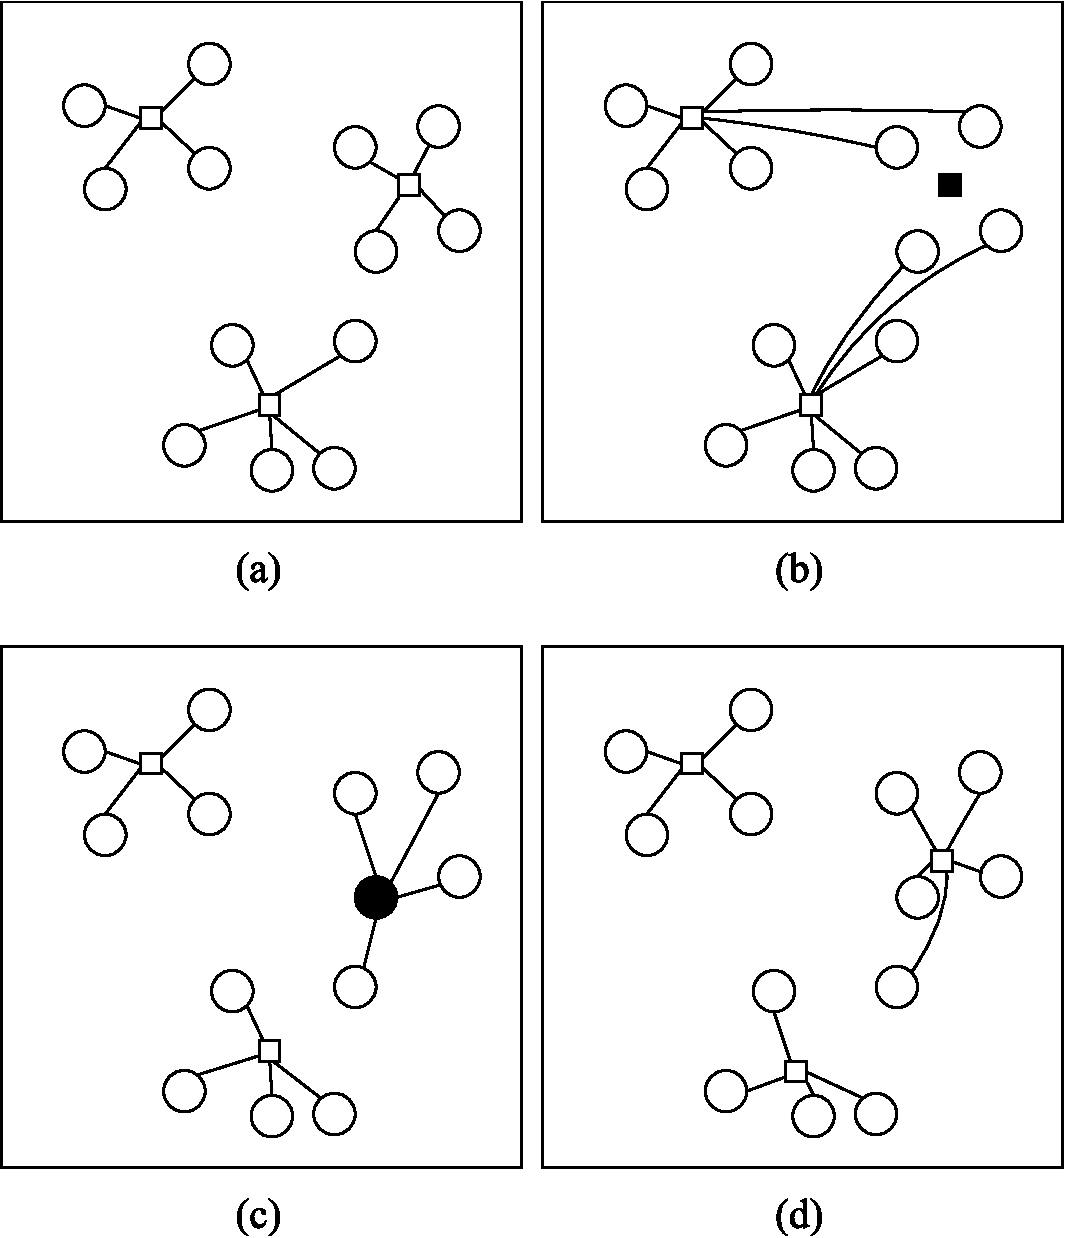
\includegraphics[width=1.0\textwidth]{img/mutation}
%    \caption{Mutation based on centroid relocation: (a) selection of the centroid to be relocated; (b) re-assignments among the remaining centroids; (c) selection of the data point where the removed centroid will be placed and (d) final re-assignments and the new solution.}\label{fig:mutation}
%  \end{center}
%\end{figure}

\begin{figure}[H]
\centering
\subfigure[Selection of the centroid to be relocated]{\label{fig:mutationA}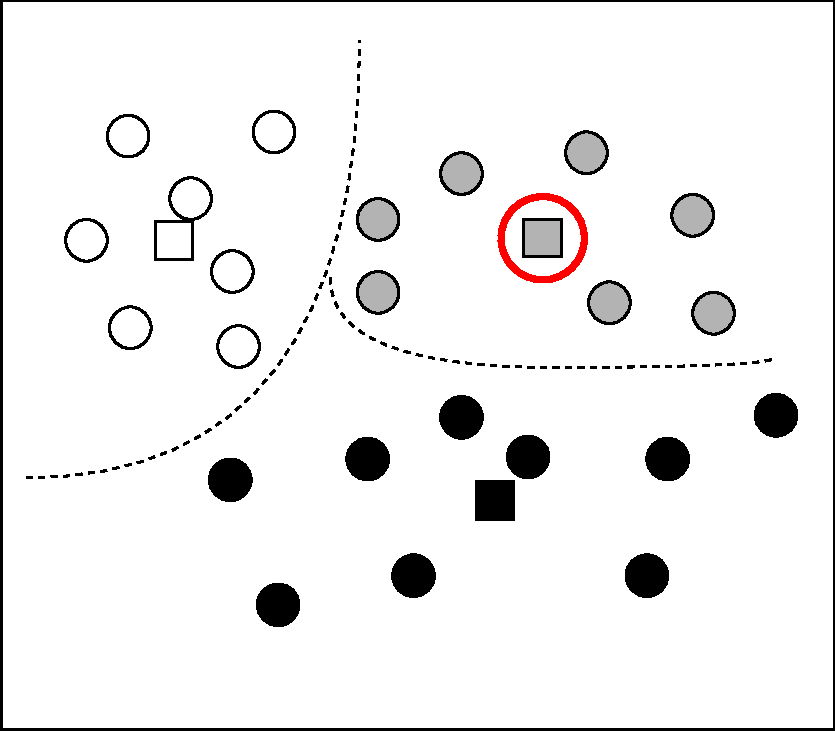
\includegraphics[width=0.4\textwidth]{img/mutationA}}
\subfigure[Re-assignments among the remaining centroids]{\label{fig:mutationB}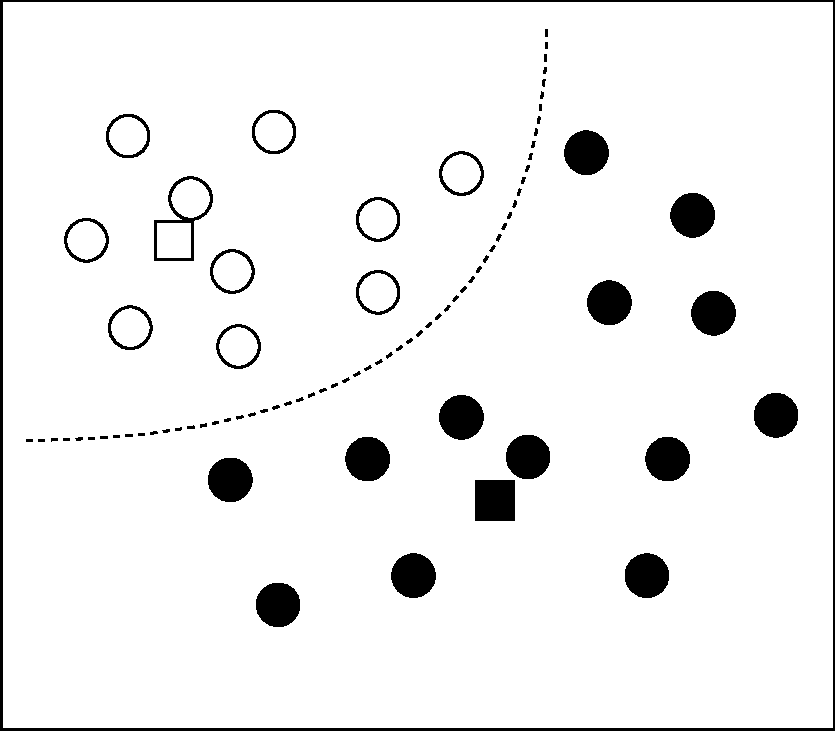
\includegraphics[width=0.4\textwidth]{img/mutationB}}
\subfigure[Selection of the data point where the removed centroid will be placed]{\label{fig:mutationC}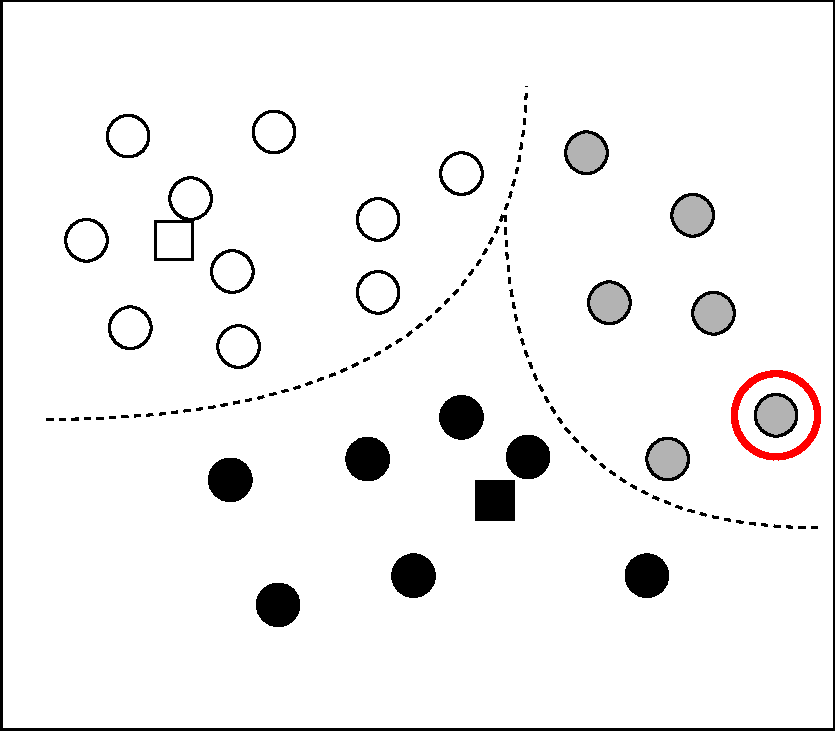
\includegraphics[width=0.4\textwidth]{img/mutationC}}
\subfigure[Final re-assignments and the new solution]{\label{fig:mutationD}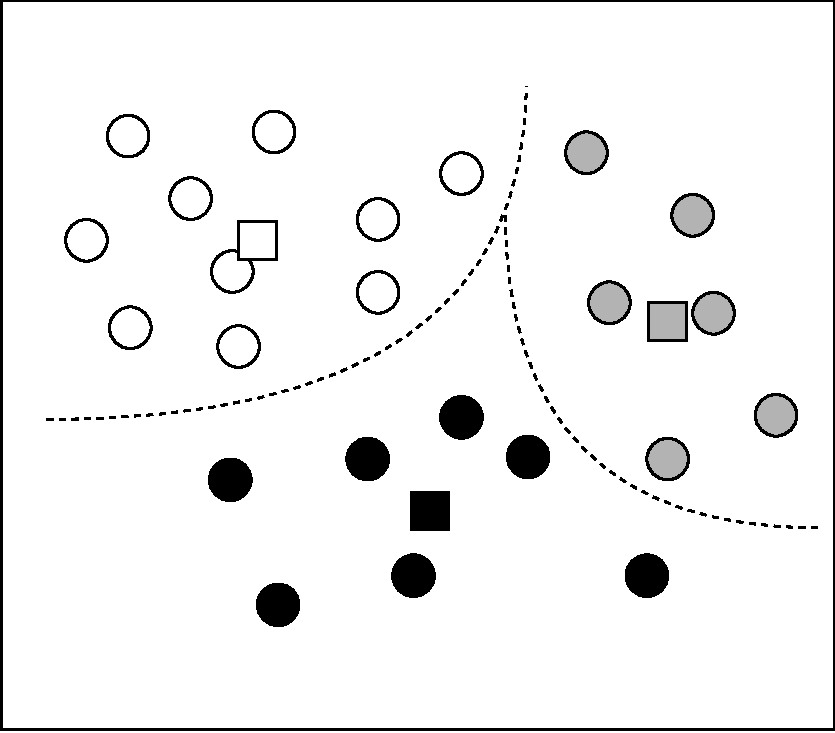
\includegraphics[width=0.4\textwidth]{img/mutationD}}
\caption{Mutation based on centroid relocation}
\label{fig:mutation}
\end{figure}

\subsection{Local improvement}
\label{subsec:local-improvement}
After the generation process in crossover and mutation, $\theta'$ is enhanced by means of a local improvement procedure. The local improvement aims to find a local optimum by applying local changes to the current solution. Here, the adopted local improvement is one run of the K-means algorithm. The K-means starts with the initial solution $\theta'$ with $m$ centroids $c_1$, $c_2$, ..., $c_m$, and proceeds by alternating between two steps:

\begin{enumerate}

	\item Assignment step: Assign each data point $x_i$ to the closest cluster.
	
	\begin{equation}
	cluster(x_i) = min_j \quad d(x_i, c_j), \quad j = 1,...,m
	\end{equation}
	
	\item Update step: Calculate the new centroids $c_j$ to be the mean (average) point of the data points in the new clusters.
	
	\begin{equation}
	c_j = \frac{\sum_{x \in S_j}x}{\left | S_j \right |}, \quad j = 1,...,m
	\end{equation}
		
\end{enumerate}

Then the algorithm keeps repeating these two steps until the assignments no longer change, converging to a local optimum.

In our experiments, we use the K-means implementation of Hamerly \cite{Hamerly2010}, who proposed an acceleration that gives the same answer of the standard Lloyd's K-means \cite{Lloyd1982} but is much faster in practice. This implementation avoids distance computations by using the triangle inequality and lower bounds on distances. The time per K-means iteration of the algorithm is O($nmd$+$md^2$), where $n$ is the number of data points, $m$ is the number of clusters and $d$ is the number of data dimensions (features). However, the calculated lower bounds allow to eliminate the innermost K-means loop in around 80\% of the time, which in practise is much faster than the standard K-means.

\subsection{Treatment of incomplete solutions}
When generating new individuals, it is possible that a cluster is left empty, i.e., no data point is allocated to it. This can happen in two situations: 

\begin{itemize}
	
	\item when generating a solution in crossover or mutation, one or more centroids could not be the closest centroid to any data point;

	\item when generating a solution in the population initialization, it could happen that some numbers in the interval [ 1, ..., $m$ ] are not chosen for the assignment, as it is a random selection.
	
\end{itemize}

To work around this issue and deal only with solutions with exactly $m$ clusters, the following procedure is adopted just after the execution of crossover, mutation and population initialization if a solution with less than $m$ clusters is generated: while there is an empty cluster, select the data point farthest from its current centroid and allocate it to an empty cluster. Important: The data point selected for relocation must belong to a cluster with more than one element, otherwise the empty cluster is populated but the cluster with one data point is left empty.

\section{Population management}
\label{sec:population-management}
One of the main challenges in population-based algorithms is avoiding premature convergence of the population. The selection of parents based on elitism favours good individuals, reducing the diversity of the genetic material in the coming generations of the population. To overcome this issue, we propose a mechanism that propagates good solutions while ensuring diversity. Thus, the search procedure can be led to unexplored regions of the search space without losing promising individuals. We call \textit{Survivors selection} as this mechanism to complement the selection, crossover and local improvement operators.

%One of the main challenges in population-based algorithms is avoiding premature convergence of the population. The selection of parents based on elitism tends to favour good individuals to mate, reducing the diversity of the genetic material in the coming generations of the population. In order to overcome this issue, we propose two mechanisms that preserve the good solutions while ensuring diversity. Thus, the search procedure can be lead to unexplored regions of the search space without losing promising individuals. We call \textit{Survivors selection} and \textit{Diversification} management as these mechanisms to complement the selection, crossover and local improvement operators.

\subsection{Survivors selection}
\label{subsec:survivors}
The \textit{Survivors selection} aims to select the best individuals to propagate when the maximum population size $\Pi$ is reached. This procedure determines the $\mu$ individuals that will go on to the next generation, by discarding $\lambda$ individuals ($\lambda = \Pi - \mu$) that are either clones (identical to other solution) or bad regarding the fitness, according to Algorithm \ref{survivors}.

This characteristic of eliminating clones and poor solutions reveals two aspects of the \textit{Survivors selection} mechanism. The first one is that population diversity is maintained, as we favour the removal of clones first. The second is related to elitism, as the individuals with good fitness are preserved. %Other aspects related to diversity can be observed in mutation and diversification operators.

\begin{algorithm}[H]
\caption{Survivors selection}
\label{survivors}
\begin{algorithmic}[1]
\FOR{$i = 1 ... \lambda$}
\STATE $X \leftarrow $ all individuals having a clone
\IF{$X \neq \emptyset$}
\STATE Remove $p \in X$ with minimum fitness
\ELSE
\STATE Remove $p$ in the population with minimum fitness
\ENDIF
\ENDFOR
\end{algorithmic}
\end{algorithm}

%\subsection{Diversification management}
%\label{subsec:diversification}
%The \textit{Diversification} mechanism aims to ensure the genetic diversity in a population. It is actually a complementary procedure to diversify the population of solutions, once the mutation carries the most important role regarding this matter. \textit{Diversification} is called after the survivors selection whenever $I_D$ iterations happen without improving the best solution. It is performed by creating $\beta$ new individuals as in the initialization phase, i.e., individuals are randomly generated and then submitted to local improvement. As this process introduces a significant amount of new genetic material, it allows the exploration of unvisited regions of the search space.

\section{Computational complexity}
\label{sec:complexity-algo}
As stated in previous sections, after the initialization of the population, the proposed meta-heuristic operates in an external loop that calls some internal operators. Among these operators, the main bottleneck is the local improvement phase, where the K-means is performed to improve the newly mutated solution. As the computational complexity of K-means is $O(nmd + md^2)$ \cite{Hamerly2010}, the overall complexity of the proposed algorithm is $O(I_{max} (nmd + md^2))$, as the local improvement is applied after the mutation in each iteration (the maximum number of iterations in the external loop is $I_{max}$). Thus, although the proposed meta-heuristic is of the same asymptotic complexity of K-means, it is in practice slower than K-means due to the constant $I_{max}$ set in the external loop and to other internal operators, like crossover, mutation, survivors selection and diversification. In the following, the computational complexity of each internal operator:

%- initial population: $O(100 * (nmd + md^2))$

%- main GA loop: $O(I_{max})$ (constant)

\begin{itemize}

	\item Selection: $O(w)$ ($w$ constant)

	\item Crossover: $O(nmd + m^{3})$

	\item Mutation: $O(nmd)$

	\item Local improvement (K-means): $O(nmd + md^2)$

\end{itemize}
%$^{*}$ $O(nmd)$ because $n$ is typically much greater than $m$, but for $n < m$ the crossover complexity becomes $O(m^{3})$ due to the Hungarian algorithm for finding the matching between centroids.

%In addition to the above internal operators, the mechanisms for population management are also performed in the general loop. However, unlike the other operators, \textit{Survivors selection} and \textit{Diversification} are not performed on each iteration, but only when some criteria are reached. \textit{Survivors selection} is performed whenever the population reaches $\Pi$ individuals; and \textit{Diversification} is called after the \textit{Survivors selection} if $I_D$ iterations happen without improving the best solution. Therefore, their contribution to the computational time of the algorithm is small in practice. Their complexities are:

In addition to the above internal operators, a mechanism to select the best individuals for propagation is also performed in the general loop. However, unlike the other operators, the \textit{Survivors selection} is not performed on each iteration, but only when the population reaches $\Pi$ individuals. Therefore, its contribution to the computational time of the algorithm is small in practice, being $O(n\frac{I_{max}}{\Pi})$.